\documentclass[12pt]{article}
%\documentclass[12pt,a4paper]{article}
%Size -- the best choice for university course
%slides seems landscape A5, 12pt letters.  Margins
%are made narrow, as much text on each page as possible.

%Could define size explicitly, but finally A5 was selected:

\usepackage[%paperwidth=600pt,paperheight=450pt,
a5paper,left=15pt,right=15pt,top=3pt,bottom=3pt,%
  %outer=25mm,
  %inner=35mm,
  %vmargin=2mm,
  includehead,includefoot,headheight=15.4pt,headsep=5pt,%
  footskip=22pt,landscape]{ geometry }


\usepackage{tocloft}
%\usepackage{tocloft}% http://ctan.org/pkg/tocloft
\setlength{\cftsecnumwidth}{1.9em}
\setlength{\cftsubsecnumwidth}{2.95em}
\setlength{\cftsubsubsecnumwidth}{3.7em}
% Set length of number width in ToC
% so that the number has enough space and
% does not run into the subsection title.

\usepackage[unicode,colorlinks=true,breaklinks]{hyperref}
%\usepackage[dvips]{hyperref}
%should display links, but it does not work with \H accent
%and formulas in section titles

\hypersetup{colorlinks,linkcolor=blue,urlcolor=magenta,citecolor=magenta}
%Breaks long url`s in text, while keeping it one link:
\usepackage{breakurl}

\newcommand{\nc}{\newcommand} % a newcommand rövidítése
\newcommand{\rc}{\renewcommand} % a renewcommand rövidítése

\newcommand{\bb}[1]{\mathbf{#1}}
\newcommand{\dd}{\mathrm{d}}

%Creates header and footer w time, section titles, etc. 
%Here the stripes are made narrow. 
\usepackage{fancyhdr}
\usepackage[yyyymmdd,hhmmss]{datetime}

\pagestyle{fancy}
\rc{\headrulewidth}{0.3pt}
\rc{\footrulewidth}{0.3pt}
%\lfoot{\today\, \currenttime}
\cfoot{}
\rfoot{\thepage}

\sloppy %To prefer larger spaces between 

%words rather than overflow a line. 
\frenchspacing %No wide space after period, this is the
%French and also the Hungarian rule. 

\usepackage{bookmark}
\usepackage[medium,compact,toctitles]{titlesec}
\usepackage[active]{srcltx}
\usepackage{braket}
%\usepackage{savetrees} 
% others: 

\usepackage{t1enc}
\usepackage{amsmath, amssymb, amsfonts, amsbsy, amsthm}
\usepackage{mathtools}
\usepackage{soul} % For \st command
\let\equation\gather
\let\endequation\endgather

%\usepackage[magyar]{babel}
\usepackage[utf8]{inputenc} 
%\usepackage[pdftex]{graphicx}

\usepackage{graphicx}
%\graphicspath{{./}{kepek/}{./files/}}

\usepackage{epstopdf}
\epstopdfsetup{update}
% only regenerate pdf files when eps file is newer

% For aligning images
% \usepackage[export]{adjustbox}

\usepackage[width=.75\textwidth]{caption}
\usepackage{lmodern}%Avoid rastering for letters.  
 
% Alább definiáljuk a magyar névelőhöz illeszkedő egyenlet hivatkozást.
% A magyar csomag része \az{..} az argumentumbeli számnévhez 
% illeszkedő névelő, \Az ugyanez % nagybetűvel, ezeket használjuk 
% alább.  
\nc{\Aeqref}[1]{\Az{\eqref{#1}}}
\nc{\aeqref}[1]{\az{\eqref{#1}}}

\usepackage{bbold}
\usepackage{ulem}
\usepackage[caption=false]{subfig} 
%\usepackage{epsfig}
%\usepackage[dvips]{color}
\usepackage{accents}
\usepackage{bbold}
\usepackage{textcomp}
\usepackage{nicefrac}%\nicefrac{}{} makes frac with slash for text
\usepackage[section]{placeins} %have \FloatBarrier,
%issued automatically at section titles 

\usepackage{wrapfig} %for wrapping text around floats 
\usepackage{indentfirst}
%for indenting the first para after section title, customary in 
%Hungarian but not so in English.  
\usepackage[integrals]{wasysym} %symbols for planets 
\usepackage{upgreek}
\usepackage{bm}\usepackage{bbm}
%I experimented with those:
%\usepackage[utopia]{mathdesign}
%\usepackage[OMLmathrm,OMLmathbf]{isomath}
%\usepackage{movie15}
%\usepackage[thinlines]{easytable} % DOES NOT WORK!
%comfortable table creation
%\begin{TAB}(r,1cm,2cm)[5pt]{|l|}{|c|c|}
%(rows,min,max)[tabcolsep]{columns}{rows}
%\end{TAB}
\usepackage{braket}


\rc*\familydefault{\sfdefault}
%entire doc in sanserif for better reading from projection

%redefine paragraph to enumerate them
\setcounter{secnumdepth}{6}
\rc\theparagraph{{\it\bf\alph{paragraph}}}
\rc\thesubparagraph{{\it\bf\roman{subparagraph}}}

\makeatletter
\rc\paragraph{\@startsection{paragraph}{4}{\z@}
{-3.25ex\@plus -1ex \@minus -.2ex}%
{5pt \@plus .2ex}%
{\normalfont\normalsize\bfseries\itshape}}
\rc\subparagraph{\@startsecton{paragraph}{5}{\z@}%
{-3.25ex\@plus -1ex \@minus -.2ex}%
{5pt \@plus .2ex}%
{\normalfont\normalsize\itshape}}

% \rc*\itemize{%
%   \ifnum \@itemdepth >\thr@@\@toodeep\else
%     \advance\@itemdepth\@ne
%     \edef\@itemitem{labelitem\romannumeral\the\@itemdepth}%
%     \expandafter
%     \list
%       \csname\@itemitem\endcsname
%       {\def\makelabel##1{\hss\llap{##1}}%
%        \setlength{\itemsep}{2pt}%
%        \setlength{\parsep}{2pt}%
%        \setlength{\parindent}{7pt}}%
%   \fi}

\makeatother

%\rc{\labelitemi}{$\to$}
%\rc{\labelitemii}{$\star$}



%Az "innen következik" jel formulában 
% \nc{\ra}{ \ \ \leadsto \ \ } %Ezen kicsi a nyíl.

% \nc{\el}{\mathcal{E}}

%számozott műfajok 
%\newtheorem{hf}{\text{\it Házi feladat}}[section]
%\nc{\HF}[1]{{\hf \tc{MB}{#1}}}
% \newtheoremstyle{mystyle}
% {headspec} \thmnumber{ #1} \thmname{#2} \thmnote{#3}
% \newtheorem{gf}{\text{\it{\cya{Gyakorló feladat}}}}[section]
% \nc{\GF}[1]{{\gf #1}}
% \nc{\GFL}[2]{{\begin{gf}\label{gf:#2} #1\end{gf}}}
% \nc{\GFN}[1]{{\vspace{-0.5\baselineskip}\gf #1}}
% \newtheorem{pl}{\text{\it{{Példa}}}}[subsection]

% \usepackage{xpatch}
% \makeatletter
% \xpatchcmd{\@thm}{\thm@headpunct{.}}{\thm@headpunct{}}{}{}
% \makeatother

% \nc{\PL}[1]{{\pl \gre{#1}}}
% \nc{\PLL}[2]{{\begin{pl}\label{pl:#2} \gre{#1}\end{pl}}}
% \nc{\dl}[2]{\hfill\yel{$2016.#1  \ \blacktriangleleft \ %
% \mid \ \blacktriangleright \ 2016.#2$}}%az előadások dátumai
% \nc{\dln}[2]{\hfill\yel{$2017.#1  \ \blacktriangleleft \ %
% \mid \ \blacktriangleright \ 2017.#2$}}%az előadások dátumai



%praktikus: vb soremelés, vbn állítható, nn egyenlet végére
\nc{\vb}{\vspace{\baselineskip}}
\nc{\vbn}[1]{\vspace{#1\baselineskip}}
\nc{\nn}{\nonumber}

%\numberwithin{equation}{subsection}
\numberwithin{equation}{section}
\usepackage{cleveref}

\setlength{\parskip}{0.3\baselineskip}
%\setlength{\itemsep}{-0.3\baselineskip} --- does not work
%\setlength{\itemsep}{2pt plus2pt minus2pt} --- does not work
\AtBeginDocument{\addtocontents{toc}{\protect\setlength{\parskip}{0pt}}}
%do not loosen toc by possibly large parskip
\linespread{0.93} %compactify

%compactify
\setcounter{topnumber}{2}
\setcounter{bottomnumber}{2}
\setcounter{totalnumber}{4}
\rc{\topfraction}{0.85}
\rc{\bottomfraction}{0.85}
\rc{\textfraction}{0.15}
\rc{\floatpagefraction}{0.7}
\rc{\theHequation}{\theHsection\arabic{equation}}
%needed for hyperref


% \usepackage{movie15} % to include movies
% \usepackage{hyperref} % prerequisite for movie15 -- these do not seem 
% to work includeonly{em0.1,em1.8} % selects from include list below, 
% but uses the other aux files and keeps eq. and sec. numberings mostly 
% correct; omitting includeonly results in including all items -- then 
% \include is equivalent to \clearpage\input{file}\clearpage.
% each included file gets its own .aux file by include
% \include{em0.1} etc.

\begin{document}

%%%%%%%%%%%%%%%%%%% FIRST PAGE %%%%%%%%%%%%%%%%
\begin{center}
    \thispagestyle{empty}
    \vspace{3.0cm}
    {\LARGE Hopfield networks}
    \vspace{1.0cm}\\
    {\large Nagy Dániel}
    \vspace{1.5cm}
    \begin{figure}[h!]
        \centering
        
\includegraphics[scale=0.3]{images/elte.eps}
    \end{figure}
    \vspace{0.5cm}
\end{center}
\newpage

\newpage
\section*{Biological and technological motivation}
\section*{Motivation and history}
\begin{itemize}
    \item Your heart is a relatively simple organ: you can easily descrbe \textit{what} it does it's a pumping blood.
    \item What about Your brain? We can't even describe \textit{what} it
    \item What is seeing something?
    \item What is thinking something?
    \item \textit{How} do you decide whether you see a cat or a dog?
    \item Can we create a machine that can do similar tasks to what our brain does? (e.g. telling what can be seen on a picture)
    \item The first steps of creating artificial neural networks dates back to the early 40s (McCulloch and Pitts)\cite{pitssmcculloch}
    \item Hebbian learning was introduced in 1949 \cite{hebb2005organization}
    \item First perceptron model by Rosenblatt in 1958 \cite{Rosenblatt58theperceptron}
    \item The Hopfield network was first described in 1974 by \cite{LogicLearningHN_Arxiv}
\end{itemize}

%\setcounter{page}{2}
%\tableofcontents
\newpage
\section*{Structure of a biological neuron}
\begin{figure}[h!]
    \centering
    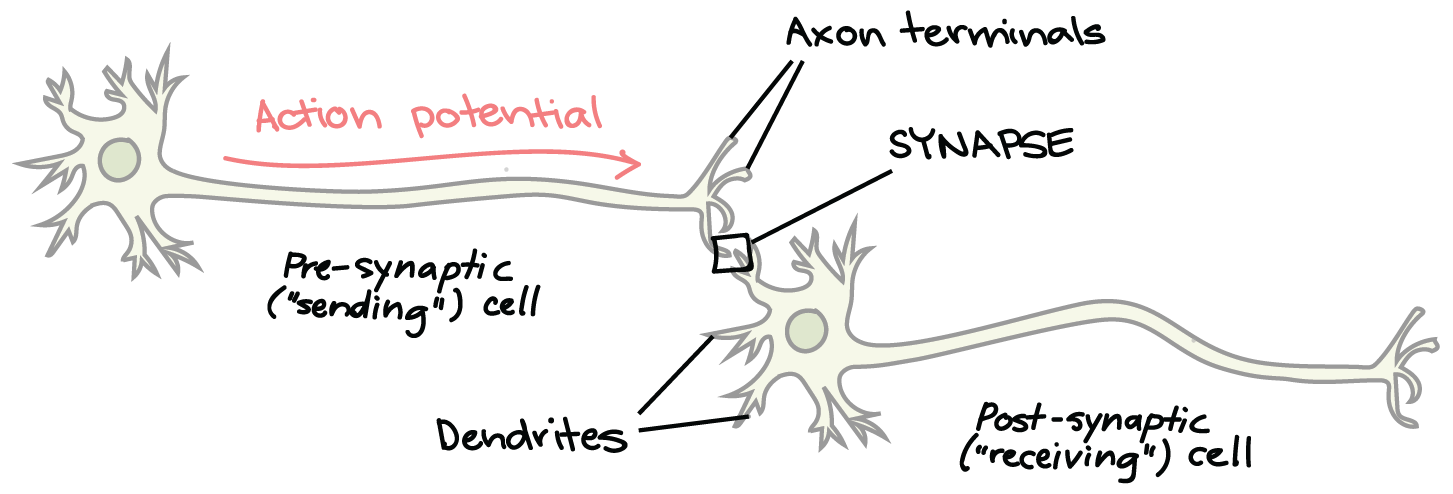
\includegraphics[scale=1.0]{images/neuron-synapse-2.png}
\end{figure}
\begin{itemize}
    \item Short story: information is carried down the axon in the form of spike-like electric pulses, and 
    transmitted through the synapse as chemical signals.
    \item inside of the cell the potential is typically $-70$mV
    \item due to the influence of the chemical signal form another neuron this potential increases a bit 
    \item If the frequency of the input signals is sufficiently large, the potential will accumulate and will reach the threshold
    \item If it reaches a threshold level of about $-55$mV, the potential flips to positive, then goes back to
    the initial level of $-70$mV
    %\item The correct biological description is more complicated an is described in \cite{geszti-neural-networks} and \cite{khanacademy_neuron}
\end{itemize}

\newpage
\section*{What happens at the synapse?}
\begin{figure}[h!]
    \centering
    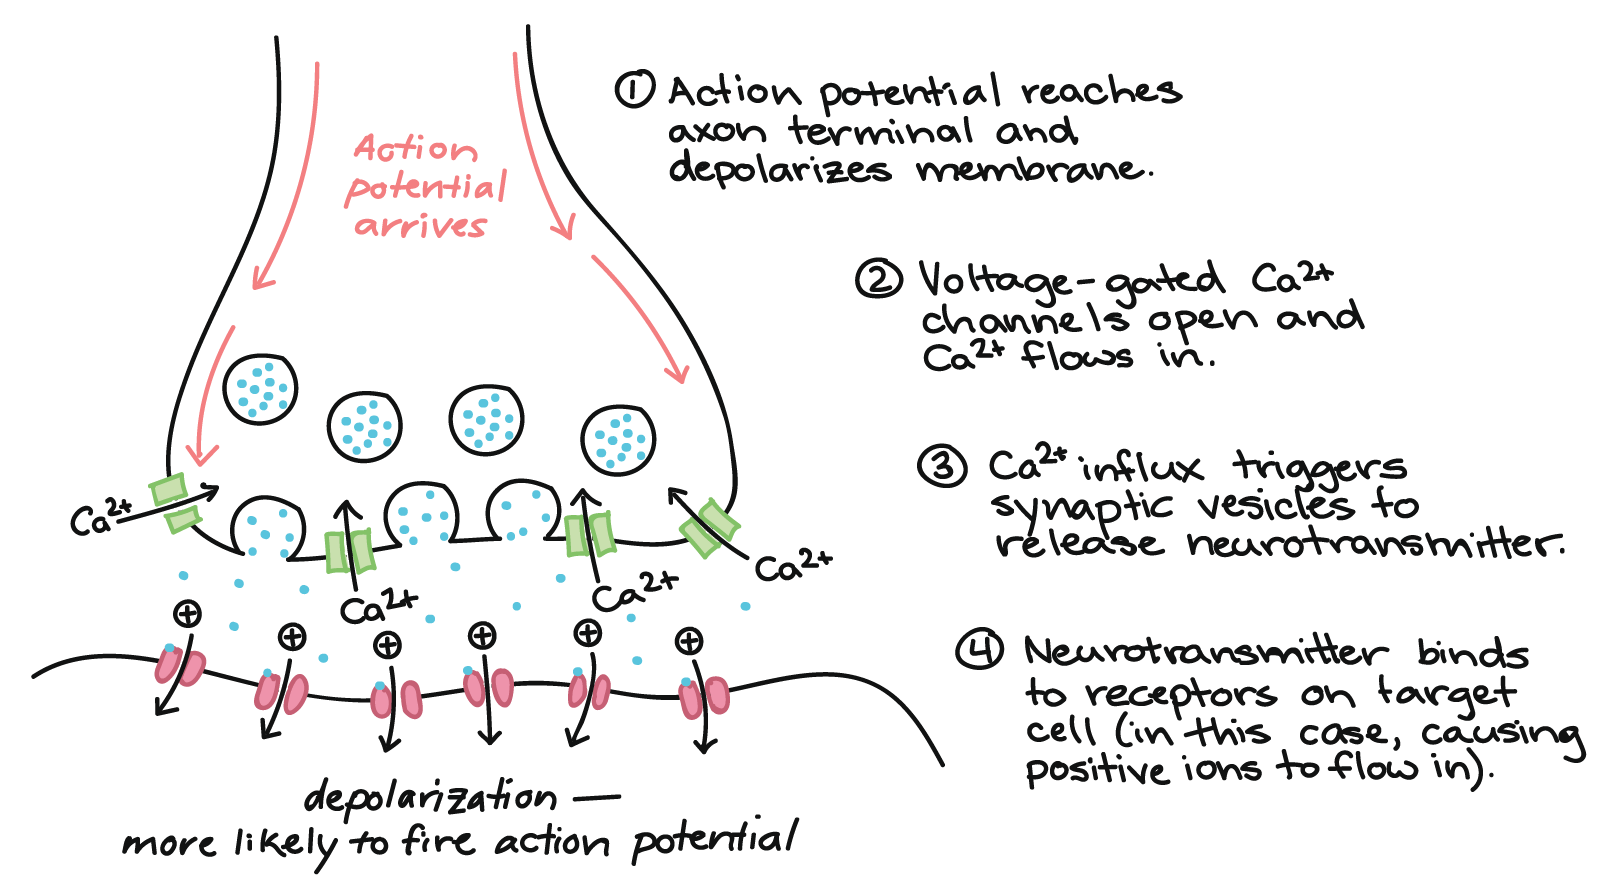
\includegraphics[height=0.8\textheight]{images/synapse-chemistry.png}
    \caption{Source: Khan Academy \cite{khanacademy_neuron}}
\end{figure}

\newpage
\begin{figure}[h!]
    \centering
    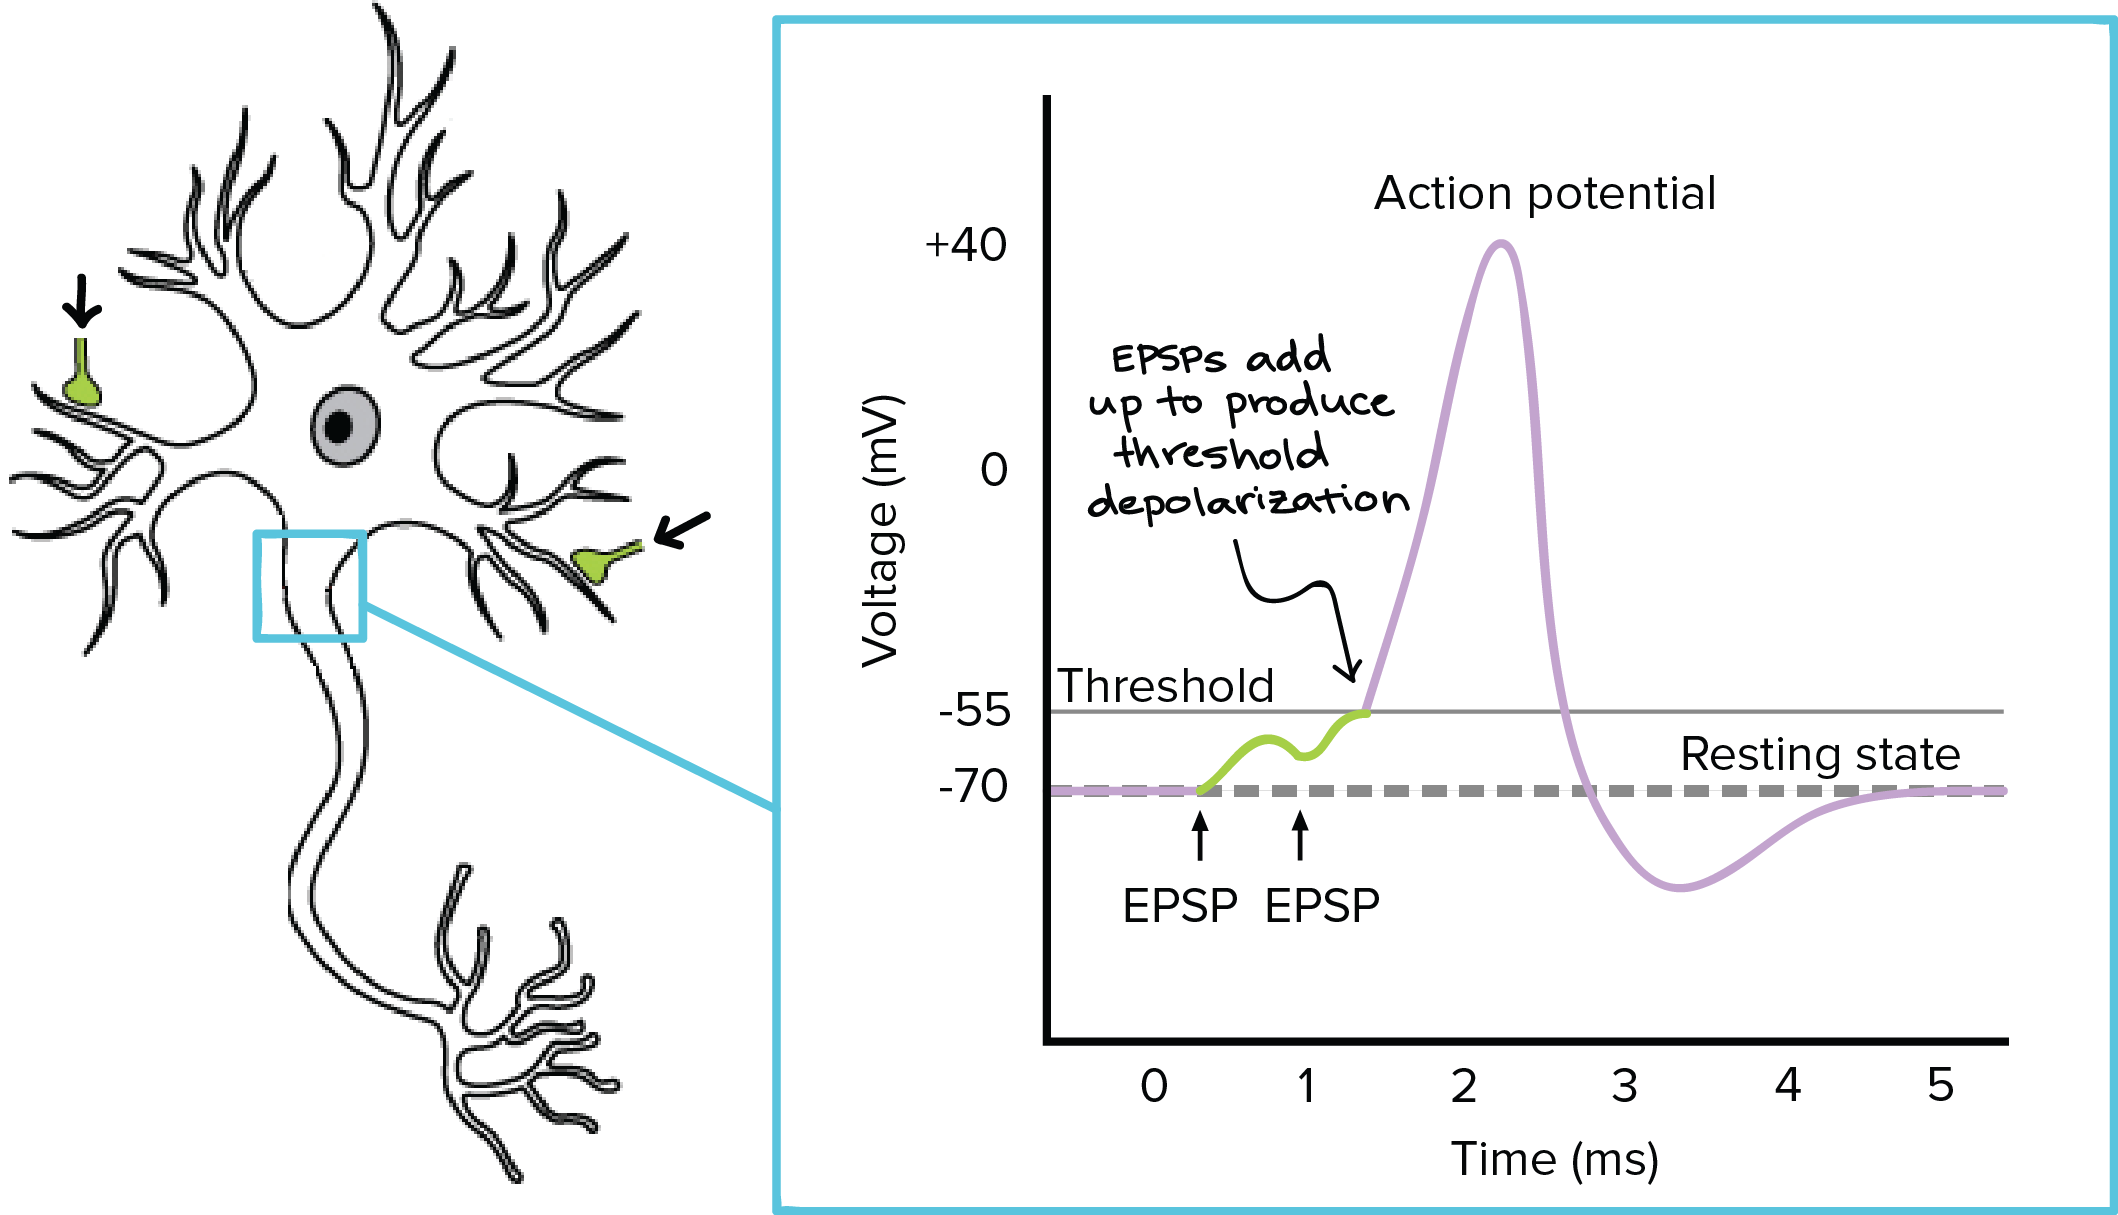
\includegraphics[height=0.6\textheight]{images/synapse-threshold.png}
\end{figure}
\begin{itemize}
    \item The output frequency $y_i$ of the $i$-th neuron depends of the input frequencies $x_j$:
    \begin{equation*}
        y_i = f\left(\sum\limits_{j}J_{ij}x_j - U\right),
    \end{equation*}
    where $U$ is the threshold potential, $J_{ij}$ are the weights descrbing the synaptic strength and 
    $f(x)$ is a filter function. 
\end{itemize}

\newpage
\begin{itemize}
    \item The filter function is usually a sigmoid, but other nonlinear activations are frequently used in machine learning.
    \item In the Hopfield-model the filter is approximated with the Heaviside step function:
    \begin{align*}
        &f_{\alpha}(x) = \frac{1}{1+e^{-\alpha x}}\\
        &f_{\infty}(x) = \Theta(x) = \begin{cases}
            1, ~\textrm{if} x > 0, \\
            0, ~\textrm{if} x \leq 0
        \end{cases}
    \end{align*}
    \item Thus a neuron has a binary state: either firing or not.
\end{itemize}
\begin{figure}[h!]
    \centering
    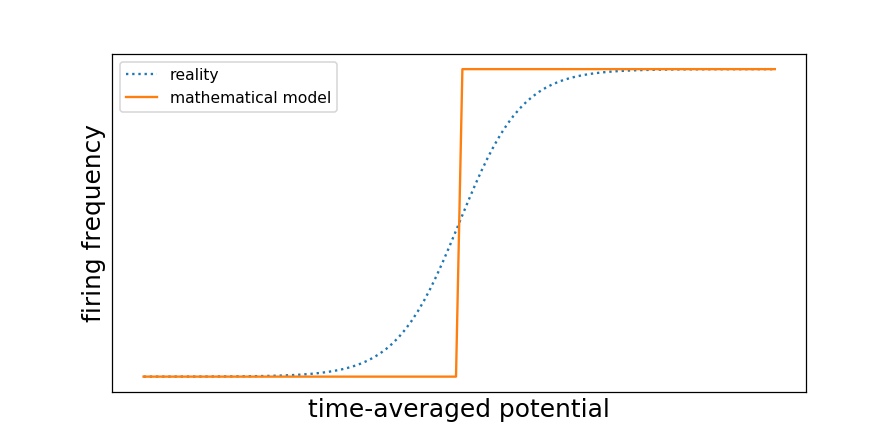
\includegraphics[height=0.5\textheight]{images/sigmoid-model.png}
\end{figure}

\newpage
\section*{Connection with the Ising-model}
\begin{itemize}
    \item $V_i(t)=$ the state of the $i$-th neuron a t $t$
    \item State update rule:
    \begin{align*}
        & V_i(t+1) = f\left(\sum\limits_{j}J_{ij}V_j(t) - U\right)
    \end{align*}
    \item Analogy with physics: neurons which are firing correspond to up spins while neurons which are 
    quiescent correspond to down spins.
    \item Introducing $S_i = 2V_i - 1 = \pm 1$, we get an Ising-model:
    \begin{align*}
        &f\left(\sum\limits_{j}J_{ij}V_j(t) - U\right) = f\left(\frac{1}{2}\sum\limits_{j}J_{ij}S_j(t)
        + \left(\frac{1}{2}\sum\limits_{j}J_{ij} - U\right)\right)
    \end{align*}
    \item Writing $J_{ij}$ instead $\frac{1}{2}J_{ij}$, this can be interpreted as 
    \begin{equation*}
        S_i(t+1) = +1,~\textrm{with probability}~f(h_i(t)),\,\textrm{where}
    \end{equation*}
    \begin{equation*}
        h_i(t) = \sum\limits_jJ_{ij}S_j(t) + \underbrace{\left(\sum\limits_jJ_{ij}-U\right)}_{h_i^{ext}}
    \end{equation*}
\end{itemize}

\newpage
\section*{Connection with the Ising-model}
\begin{itemize}
    \item The hoise level can be characterised by the inverse temperature, $\beta$
    \item In a magnetic field $h_i$, spin $i$ has energy $\varepsilon_i = -h_iS_i$
    \item The probability if the $i$-th spin to have value $S_i$ is $P(S_i) \propto e^{-\beta\varepsilon_i} = e^{+\beta h_iS_i}$
    \begin{equation*}
        \implies P\left(S_i(t+1)=+1|h_i(t)\right) = f(h_i(t)) = \frac{e^{\beta h_i(t)}}{e^{\beta h_i(t)} + e^{-\beta h_i(t)}}
        = \frac{1}{1+e^{-2\beta h_i(t)}}.
    \end{equation*}
    \item Therefore,
    \begin{equation*}
        S_i(t+1) = \begin{cases}
            +1,\,\textrm{with probability}~\frac{1}{1+e^{-2\beta h_i(t)}}\\
            -1,\,\textrm{with probability}~\frac{1}{1+e^{+2\beta h_i(t)}}
        \end{cases}
    \end{equation*}
    \item $S_i(t+1)$ tends to be parallel with $h_i(t)$
    \item The difference between probabilities vanishes as the noise $\beta\rightarrow 0$.
\end{itemize}

\newpage
\section*{Hebbian learning}
\begin{itemize}
    \item We need a model for \textit{learning} and \textit{memory}, since these are essential functions of the brain.
    \item Information can be encoded in a firing pattern $\{\xi\},\,\xi_i=\pm 1\,\textrm{for}\,(i=1,\dots, N)$.
    \item A firing pattern is stable, if the neural network comes back to this pattern after a disturbance:
    \begin{equation*}
        S_i(t) = \xi_i \rightarrow S_i(t+1)=\xi_i
    \end{equation*}
    \item The stable patterns are attractors of the dynamics of the network.
    \item Learning a pattern is achieved by setting the synaptic strengths $J_{ij}$.
    \item Hebb's rule for updating synaptic weights:
    \begin{equation*}
        J_{ij} \rightarrow J_{ij} + \lambda\xi_i\xi_j,
    \end{equation*}
    where $\lambda$ is the amplitude of learning (learning rate).
    \item This rule is extremely simple yet it proved to be very powerful.
    \item What if we want to store $p$ different patterns in the same network?
    \item We need to set $J_{ij}$ so that $\xi_i^{\mu}$ are attractors of the network dynamics for
    $\mu\in\{1,...,p\}$.
    \item The \textbf{Hopfield-network} is capable of learning $p$ different patterns using Hebb's learning Rule.
\end{itemize}

\newpage
\section*{The Hopfield network}
\begin{minipage}[c]{0.45\textwidth}
    \begin{itemize}
        \item Every node in the network has two states $S_i = \pm 1$.
        \item Every node is connected to every node, forming a complete 
        undirected weighted graph.
        \item The connection weights are $J_{ij}$ with the restrictions
        $J_{ii}=0$, $J_{ij} = J_{ji}$. 
        \item The dynamics of the network is described by
        \begin{equation*}
            S_i(t+1) = \begin{cases}
                +1,\,\textrm{if}\,\sum\limits_jJ_{ij}S_i(t) \geq U_i,\\
                -1,\,\textrm{otherwise}
            \end{cases}
        \end{equation*}
        \item The noise factor $\beta$ is assumed to be $0$.
        \item It works as a content-addressable memory a.k.a. associative memory.
        \item Interestingly, it can reconstruct data after being fed with corrupt versions of the same data.
        \item Can be trained using the Hebbian training rule.
    \end{itemize}
\end{minipage}
\hfill
\begin{minipage}[c]{0.45\textwidth}
    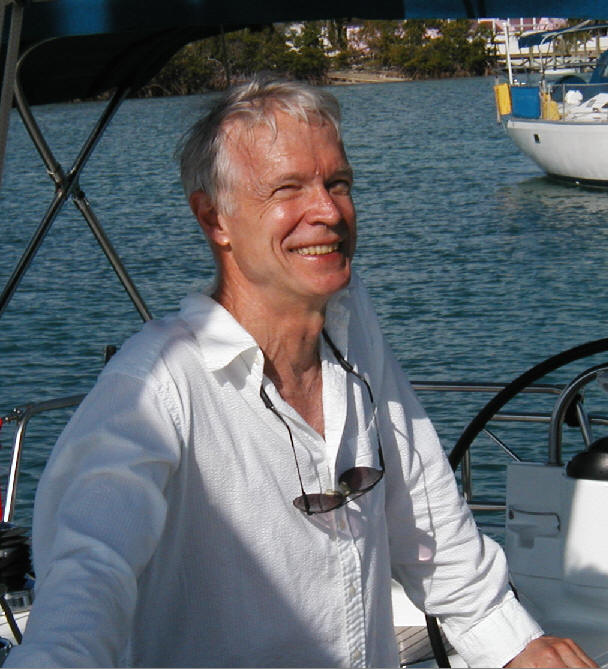
\includegraphics[width=\textwidth]{./images/JJHopfield.png}
    \begin{center}
        {\texttt{John Joseph Hopfield (1933-)}}
    \end{center}
\end{minipage}

\newpage
\section*{Hebbian learning in Hopfield-networks}
\begin{itemize}
    \item Motto: \textit{"Neurons that fire together, wire together. Neurons that fire out of sync, fail to link."}
    \item Suppose, we have $p$ different patterns $\xi^{\mu}_1, \dots, \xi^{\mu}_N \in \{\pm 1\}$, for $\mu \in \{1,\dots,p\}$
    \item Then we can set the weights (initially $J_{ij}=0$) with the Hebbian rule:
    \begin{equation*}
        J_{ij} = \lambda\sum\limits_{\mu=1}^{p}\xi^{\mu}_i\xi^{\mu}_j~\textrm{for}~i\neq j~\textrm{and}~J_{ii}=0,
    \end{equation*}
    where $\lambda$ is usually set to $1/p$.
    \item We can define an energy-like scalar value for each state of the network:
    \begin{equation*}
        E = -\frac{1}{2}\sum\limits_{i,j}J_{ij}S_iS_j + \sum\limits_iU_iS_i
    \end{equation*}
    \item Under repeated updating the network will eventually converge to a state which is a
    local minimum in the energy function.
    \item If a state corresponds to a local minimum of the energy function, it is a stable state of the network.
    \item The states $\{\xi_i^{\mu}\}$ are attractors of the dynamics thus they are stable states of the network and
    their corresponding energy level is a local minimum.
\end{itemize}

\newpage
\section*{Data reconstruction}
% \begin{figure}[h!]
%     \centering
%     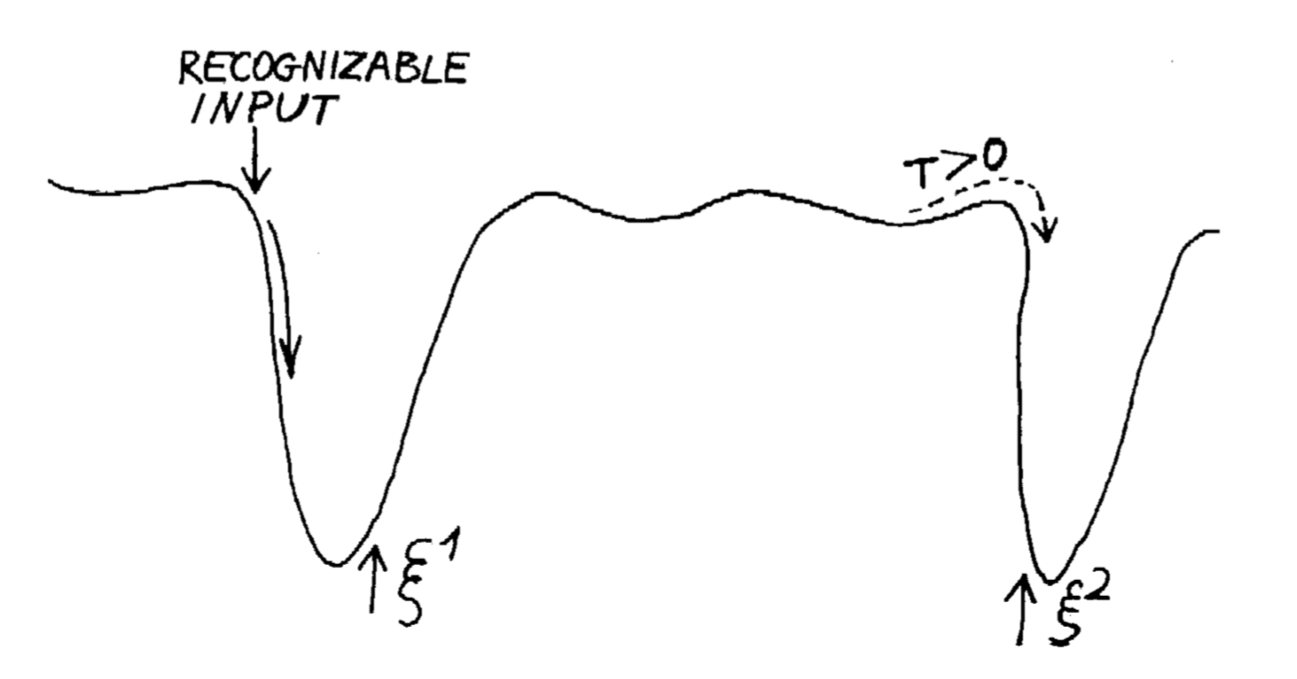
\includegraphics[height=0.5\textheight]{images/hopfield-energy-plot.png}
% \end{figure}
\begin{figure}[h!]
  \centering
  \begin{minipage}{0.69\textwidth}
    \centering
    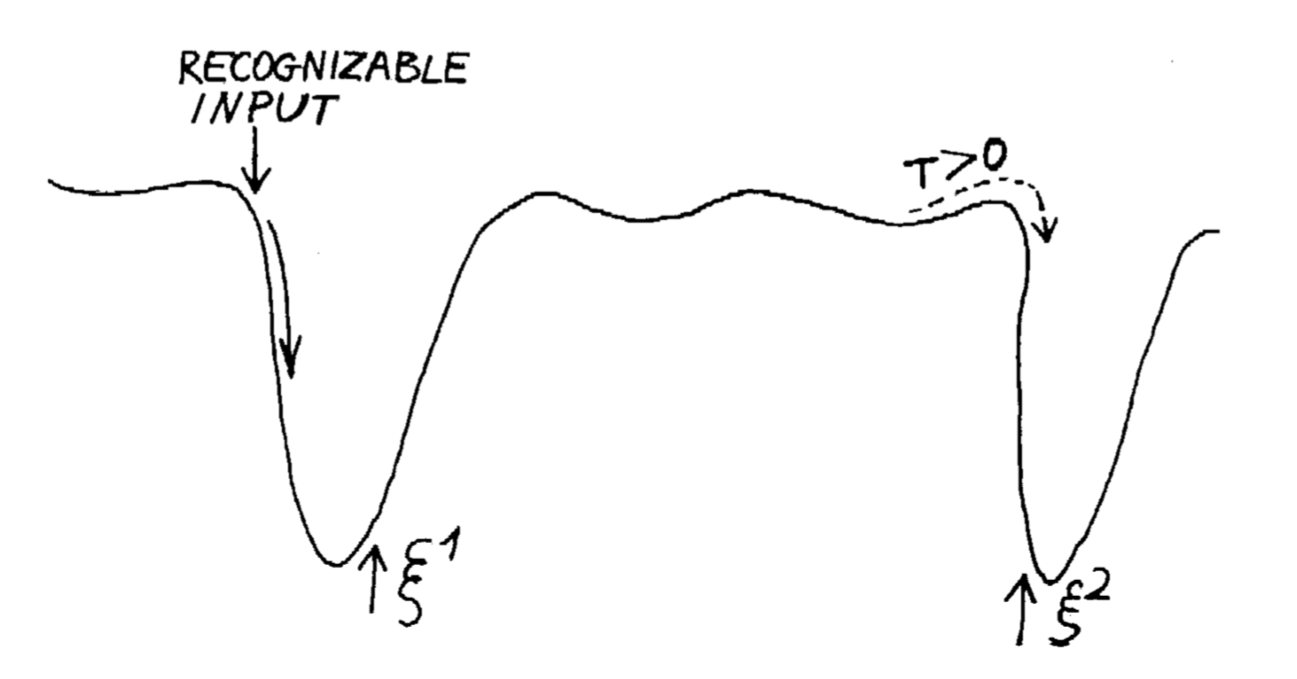
\includegraphics[width=1.0\textwidth]{./images/hopfield-energy-plot.png} % second figure itself
    %\caption{second figure}
\end{minipage}\hfill
  \begin{minipage}{0.29\textwidth}
      \centering
      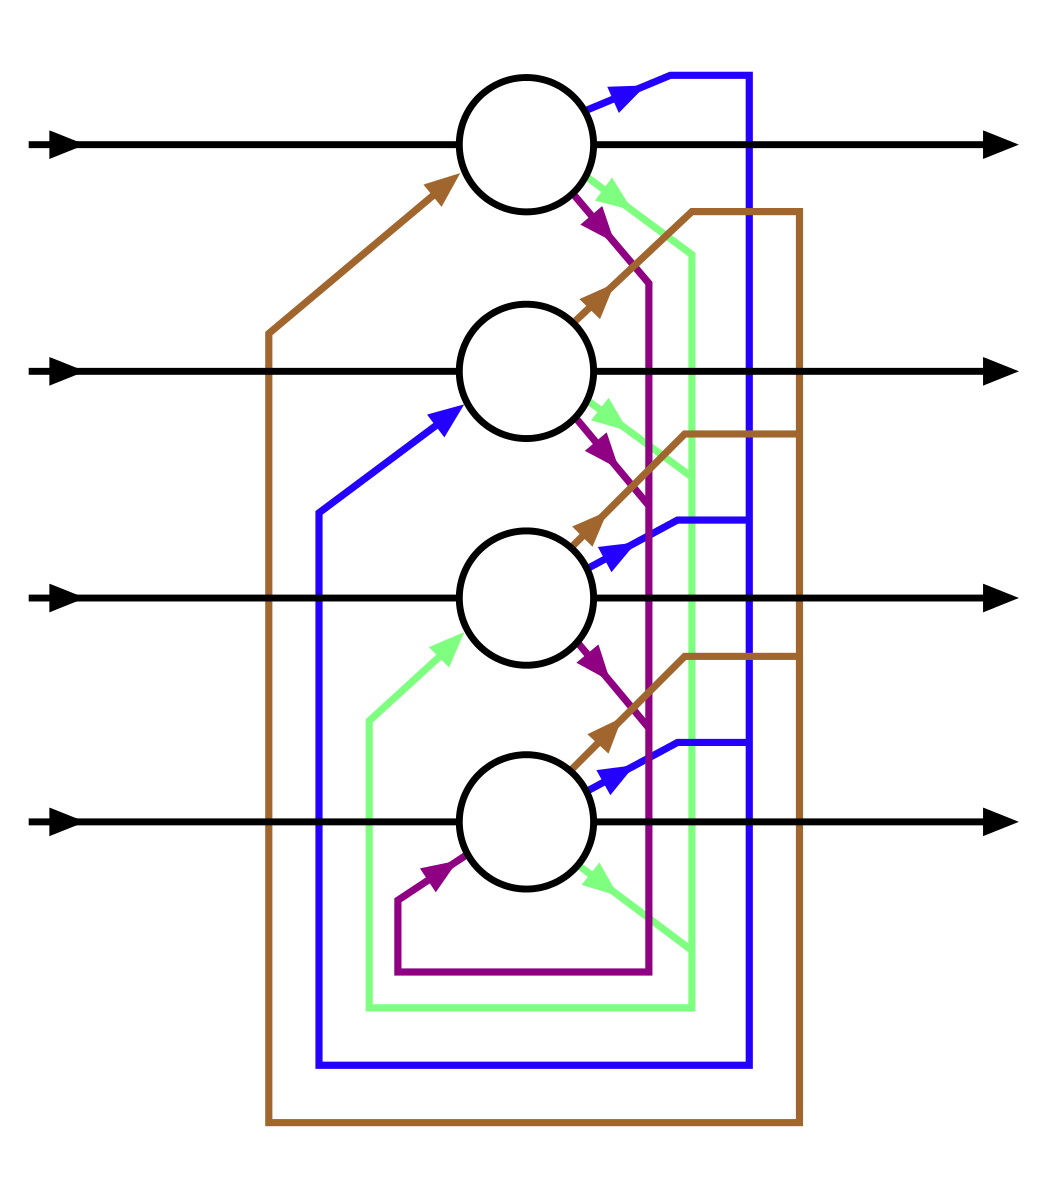
\includegraphics[width=1.0\textwidth]{./images/Hopfield-net-vector.png} % first figure itself
      %\caption{first figure}
  \end{minipage}
\end{figure}
\begin{itemize}
    \item If we give a corrupted input, the systems dynamics will drive the network to the
    nearest local minima, which is hopefully the reconstructed data.
\end{itemize}

\newpage
\section*{Data reconstruction}
\begin{figure}[h!]
    \centering
    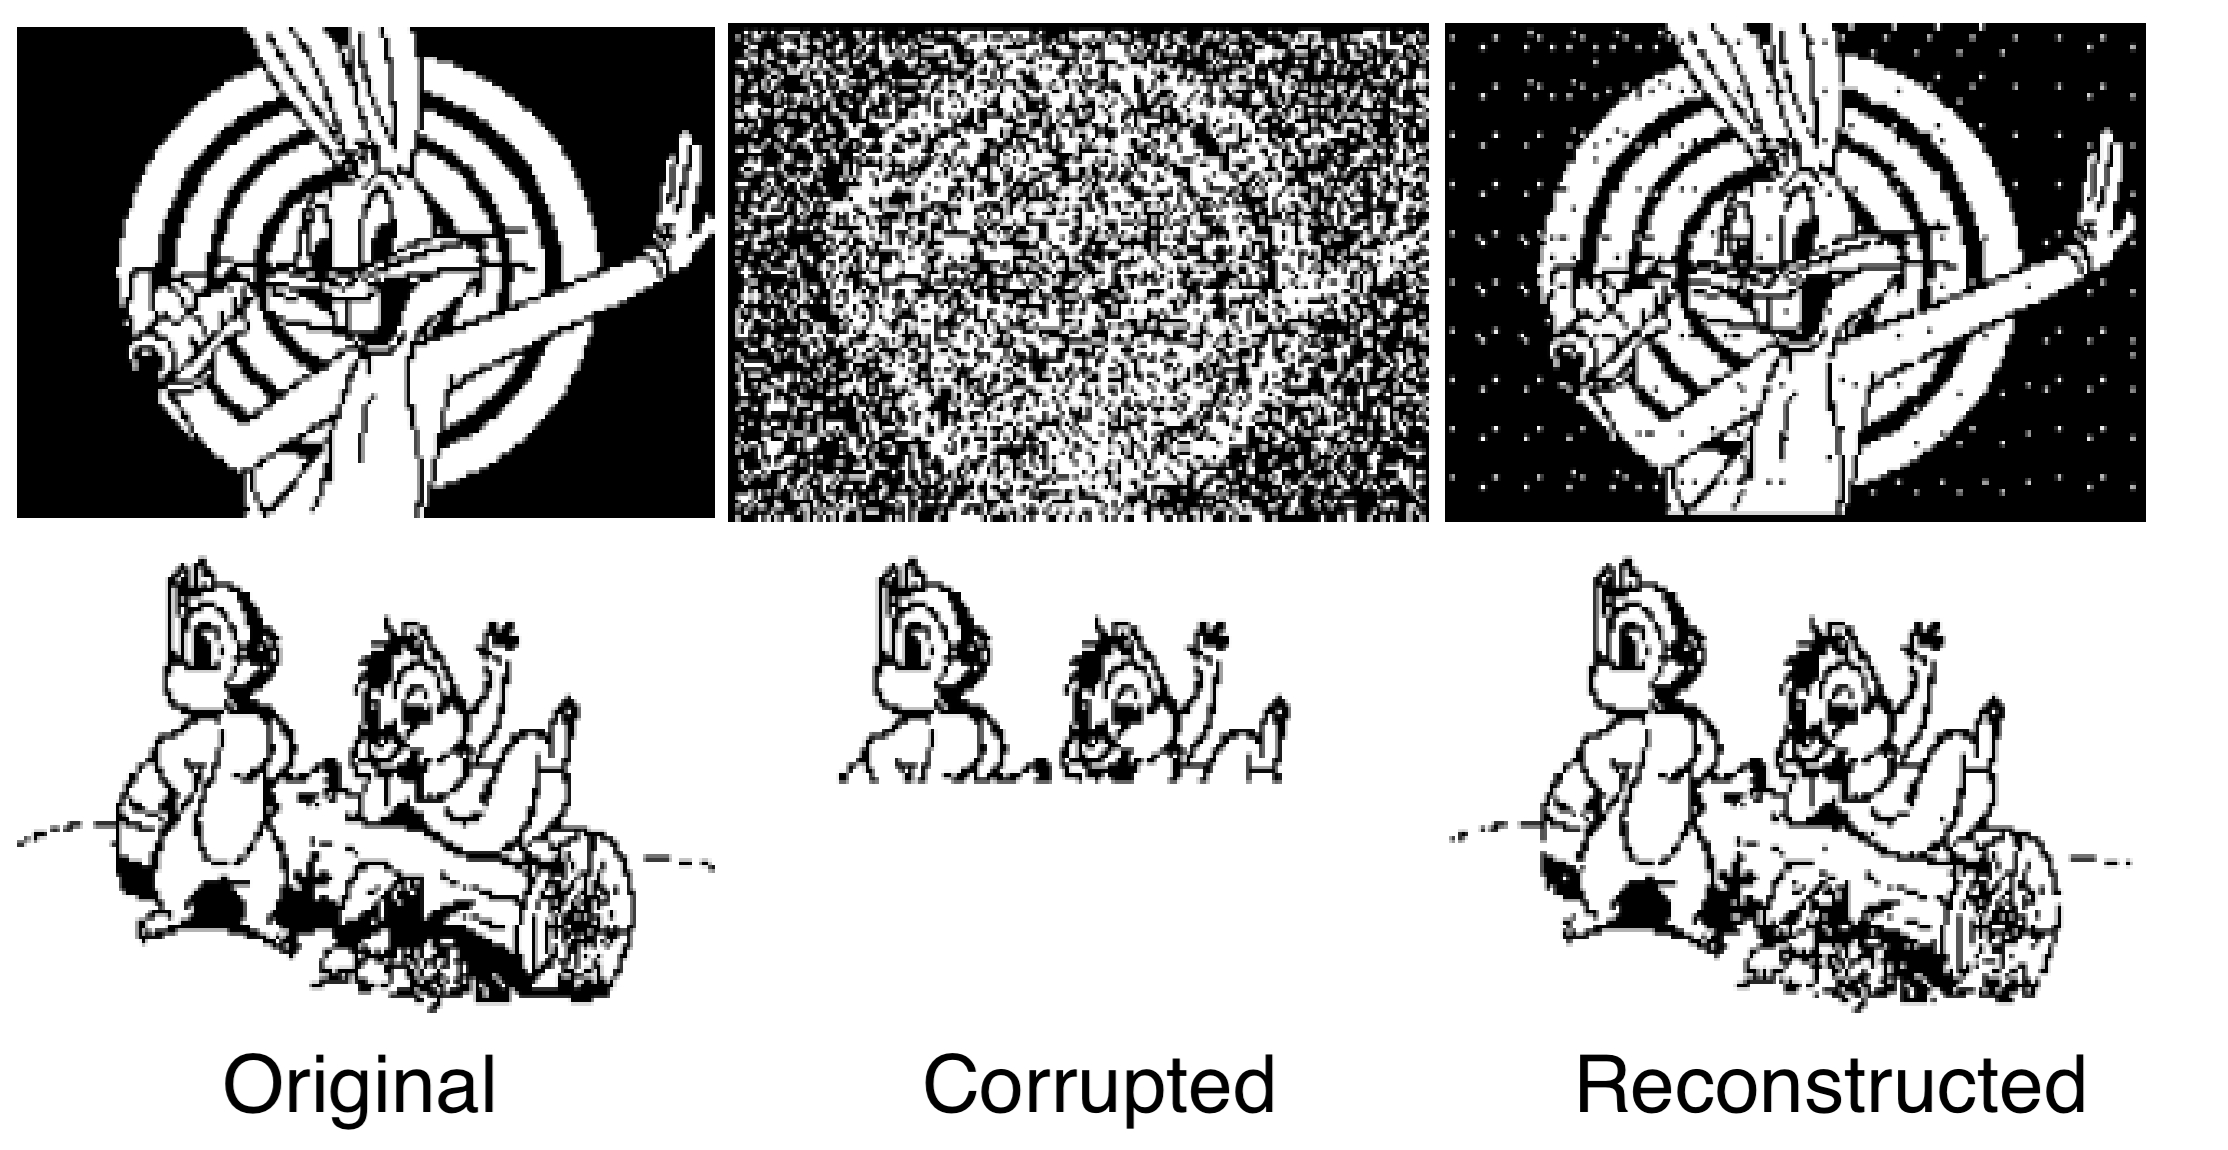
\includegraphics[height=0.5\textheight]{images/hopfield-reconstruction.png}
\end{figure}
\begin{itemize}
    \item If we give a corrupted input, the systems dynamics will drive the network to the
    nearest local minima, which is hopefully the reconstructed data.
\end{itemize}

\newpage
\section*{Storkey learning rule}
\begin{itemize}
    \item Another useful rule for learning is the \textit{Storkey-learning rule}:
    \begin{equation*}
        J_{ij} \rightarrow J_{ij} + \frac{1}{p}\xi_i^{\mu}\xi_j^{\mu} - \frac{1}{p}\xi^{\mu}_i h^{\mu}_j - \frac{1}{p}\xi^{\mu}_j h^{\mu}_i,
    \end{equation*}
    where
    \begin{equation*}
        h^{\mu}_i = \sum\limits_j J_{ij}S_i^{\mu}.
    \end{equation*}
    \item Hopfield-networks trained with the Hebbian rule have capacity $\approx 0.138$ i.e. they can store $138$
    different patterns per 1000 nodes.
    \item Networks trained with the Storkey rule have capacity $\geq 0.14$ \cite{Liou1999}.
    \item There exist higher-order Storkey learning rules and many other tricks for increasing the capacity of 
    Hopfield-networks \cite{aboudib:hal-01058303}.
\end{itemize}

\newpage
\section*{Quantum Hopfield networks}
\begin{itemize}
    \item Over the past few decades, quantum information science became reality rather than a physicists' utopy.
    \item Many quantum devices are accessible to experimentalists and the quantum hype is huge.
    \item Given the fact that artificial neural networks have made a huge impact in computer science,
    and quantum computing seems feasible, scientists started talking about quantum machine learning.
    \item In 2018, the quantum version of the Hopfield networks was described by Patrick Rebentrost et. al. \cite{quantum-hopfield}
    \item Why quantum Hopfield-nets?
    \item An exponentially large network can be stored in a polynomial number of quantum bits by encoding the network into the amplitudes of quantum states.
    \item Using quantum algorithms a computational complexity that is logarithmic in the dimension of the data can be achieved.
    \item The quantum Hopfield network can be used as a genetic sequence recognizer.
\end{itemize}

\newpage
\section*{Quantum Hopfield networks}
\begin{itemize}
    \item The d-dimensional information is encoded in d-level quantum states:
    \begin{equation*}
        \mathbf x = \{x_1,\dots,x_d\}\rightarrow |\mathbf x|_2\ket x,
    \end{equation*}
    where 
    \begin{equation*}
        |\mathbf x|_2 = \sqrt{\sum\limits_{i=1}^d x_i^2}~\textrm{and}~\ket x = \frac{1}{|\mathbf x|_2}\sum\limits_{i=1}^dx_i\ket i.
    \end{equation*}
    \item this $d$-level quantum system can be implemented using $N=\log_2 d$ qubits, so qubit representation of the network
    scales logarithmically with the number of neurons \cite{quantum-hopfield}.
    \item training items $\mathbf x^{(m)}$ can be associated with pure states $\ket{x^{(m)}}$.
    \item A weight matrxi $W$ can be associated to the mixed state $\hat \rho$:
    \begin{equation*}
        \hat \rho = \frac{1}{M}\sum\limits_{m=1}^M\ket{x^{(m)}}\bra{x^{(m)}} = W + \frac{\mathbb 1_d}{d}.
    \end{equation*}
    \item This state $\rho$ then can be used to retrive states $\ket{x^{(m)}}$ using quantum state tomography and other tricks \cite{quantum-hopfield}.
    \item It was showed that the quantum Hopfield network outperforms the classical HN in RNA sequence recognition. \cite{quantum-hopfield}.
    \item The bottlenecks of the quantum Hopfield network are pure state preparation and state tomography at readout.
    \item It can be still exponentially better in time complexity than the classical Hopfield network.
\end{itemize}

\newpage
\section*{Conclusion}
\begin{itemize}
    \item The Hopfield-network was one of the earliest and simplest form of neural networks.
    \item The Hopfield network can act as a non-sequential associative memory,
    with technological application in image processing and optimization.
    \item Hopfield networks can be trained with the Hebbian training rule which is fairly simple.
    \item Other, more advanced training rules exist.
    \item Hopfield networks are not competitive with the modern neural networks, which apply 
    many hidden layers and are trained with automatic differentiation and backpropagation.

\end{itemize}
%%%%%%%%%%%%%%%%%%%%%%%%%%%%%%%%%%%% END OF RIZSA %%%%%%%%%%%%%%%%%%%%%%%%%%%

%%%%%%%%%%%%%%%%%%%%%%%%%%%%%%%%%%%%%%%%  PAGE WITH 2 FIGURES  %%%%%%%%%%%%%%%%%%%%%%%%%%%%%%%%%
% \newpage
% \section*{Defining a simple square lattice}
% \begin{figure}[h!]
%   \centering
%   \begin{minipage}{0.49\textwidth}
%     \centering
%     \includegraphics[width=1.0\textwidth]{./media/example-1-code.png} % second figure itself
%     \caption{second figure}
% \end{minipage}\hfill
%   \begin{minipage}{0.49\textwidth}
%       \centering
%       \includegraphics[width=1.0\textwidth]{./media/example-1.png} % first figure itself
%       \caption{first figure}
%   \end{minipage}
% \end{figure}

%%%%%%%%%%%%%%%%%%%%%%%%%%%%%%%%%%%%%%%  SINGLE FIGURE  %%%%%%%%%%%%%%%%%%%%%%%%%%%%%%%%%%%%%
% \begin{figure}[h!]
%     \begin{center}
%         \includegraphics[height=0.7\textheight]{./media/2degconst_W8_L10.png}
%         \caption{2DEG system: a point contact}
%         \label{fig:2degconst}
%     \end{center}
% \end{figure}

\newpage
\phantomsection

%%%%%%%%%%%%%%%%%%%%%%%%%%%%%%%%%%%%%%%  Bibliography  %%%%%%%%%%%%%%%%%%%%%%%%%%%%%%%%%%%%%
\newpage
\nocite{*}
\bibliographystyle{plain}
\bibliography{references}

%%%%%%%%%%%%%%%%%%%%%%%%%%%%%%%%%%%%%%%  Last page  %%%%%%%%%%%%%%%%%%%%%%%%%%%%%%%%%%%%%
\newpage
\newpage
\thispagestyle{empty}
\topskip0pt
\vspace*{\fill}
\begin{center}
    \LARGE{Thank You for listening!}
\end{center}
\vspace*{\fill}


\end{document}
